\documentclass{article}
\usepackage[latin1]{inputenc}
\usepackage{amsfonts}
\usepackage{epsfig}
\usepackage{hyperref}
\usepackage{multicol}
\usepackage{graphicx}
\usepackage{color}
\usepackage[margin=1in]{geometry}
\usepackage{setspace}



\usepackage{tikz}
\usetikzlibrary{backgrounds}
\makeatletter

\tikzset{%
  fancy quotes/.style={
    text width=\fq@width pt,
    align=justify,
    inner sep=1em,
    anchor=north west,
    minimum width=\textwidth,
  },
  fancy quotes width/.initial={.8\textwidth},
  fancy quotes marks/.style={
    scale=8,
    text=white,
    inner sep=0pt,
  },
  fancy quotes opening/.style={
    fancy quotes marks,
  },
  fancy quotes closing/.style={
    fancy quotes marks,
  },
  fancy quotes background/.style={
    show background rectangle,
    inner frame xsep=0pt,
    background rectangle/.style={
      fill=gray!25,
      rounded corners,
    },
  }
}

\newenvironment{fancyquotes}[1][]{%
\noindent
\tikzpicture[fancy quotes background]
\node[fancy quotes opening,anchor=north west] (fq@ul) at (0,0) {``};
\tikz@scan@one@point\pgfutil@firstofone(fq@ul.east)
\pgfmathsetmacro{\fq@width}{\textwidth - 2*\pgf@x}
\node[fancy quotes,#1] (fq@txt) at (fq@ul.north west) \bgroup}
{\egroup;
\node[overlay,fancy quotes closing,anchor=east] at (fq@txt.south east) {''};
\endtikzpicture}

\makeatother


\setstretch{1.35}





\title{A postcolonial view of \emph{The Tempest} and its Afterlives}

\author {Ravi Bhoraskar}
\begin{document}
\maketitle
\begin{abstract}
  We discuss William Shakespeare's last play, \emph{The Tempest} along with three of its afterlives, Neil Gaiman's graphic novel \emph{The Tempest}, \emph{The Tempest: Graphic Novel} and Charles Lamb's adaptation of the play in \emph{Tales from Shakespeare}. We view these pieces through the lens of postcolonial theory, and comment on the plot, the setting and the characters.
\end{abstract}
\section{Introduction}
\subsection{A brief history of British Colonization}
Let us begin our discussion with a brief history of British Colonization. This will help us understand the historical and social context when Shakespeare wrote \emph{The Tempest}. Christopher Columbus was searching for a western sea route to India, when he discovered America in 1492. In 1497, Henry VII commissioned John Cabot to sail west, and he became the first Englishman to set foot on American soil. Notice that so far there was no colonization, and new lands were discovered with the purpose of trade and getting natural resources. It was only 1576 onwards that the early claims of land in the name of the queen began to be made. British colonization of America started in 1607, when the \emph{Virginia Company} set up a colony in the town of Jamestown, Virginia. Thus, when Shakespeare wrote \emph{The Tempest} in 1611, colonization was fairly recent and in the public consciousness. However, the parallels that are drawn between \emph{The Tempest} and the Colonial Discourse are more likely to be prophetic rather than descriptive, since colonization was not old enough yet for all its complexities and moral issues to be revealed.

An incident that is likely to be Shakespeare's inspiration for \emph{The Tempest} took place in 1609. A ship called the \emph{Sea Venture} was commissioned to deliver supplies to the British Colony in Jamestown, Virginia. The ship set sail on June $20^{th}$, but unfortunately ran into a storm and sank on July $24^{th}$. However, all 150 passengers safely landed ashore onto a coral reef in Bermuda, where they remained stranded for nine months. Eventually, they built two new boats and set sail to Virginia where most of the 150 passengers landed alive. The accounts of this seemingly miraculous event were written by \emph{William Strachey}, and are considered another inspiration for \emph{The Tempest}.

\subsection{The Tempest}
\emph{The Tempest} is William Shakespeare's last play, written in 1610-11. It is the one of the only two Shakespearean plays that seem to be entirely original, the other being \emph{A Midsummer Night's Dream}. The plot is based in the Mediterranean, but the description of the island seems more reminiscent of the \emph{New World}, which was being colonized when this play was written. In contrast to other Shakespearean plays, \emph{The Tempest} strictly observes the three unities of time, place and action. Critics have seen Prospero as an image of Shakespeare, with his renunciation of magic at the end of the play depicting Shakespeare's farewell to the stage. Due to space constraints, I shall not include a summary of the text here, but shall direct the interested reader to ~\cite{tempest} and ~\cite{lamb}. 

%% \subsection{The Afterlives}
%% %This section probably isn't required
%% We shall discuss three afterlives of \emph{The Tempest}. The first one is \emph{The Tempest}, by Neil Gaiman ~\cite{gaimantempest}. This is the last book of the 

%% \subsection{The Afterlives}
%% \begin{frame}{The Afterlives}
%%   \begin{enumerate}
%%   \item \textbf{Neil Gaiman's \emph{The Tempest}}~\cite{gaimantempest}
%%     \begin{itemize}
%%     \item \textbf{1997} Last book of \emph{The Sandman} series, part of \emph{The Wake}
%%     \end{itemize}
%%   \item \textbf{Charles and Mary Lamb's \emph{Tales from Shakespeare} }~\cite{lamb}
%%     \begin{itemize}
%%     \item \textbf{1807} Written as an abridged version of Shakespeare for children
%%     \item Attempts to be a reproduction, but is an afterlife, due to cultural sensibilities of its times
%%     \end{itemize}
%%   \item \textbf{The Tempest: Graphic Novel}~\cite{tempestgraphicnovel}
%%     \begin{itemize}
%%     \item \textbf{2009} Retains the original text, but adds pictures
%%     \end{itemize}
%%   \end{enumerate}
%% \end{frame}

\section{Postcolonial Theory and The Tempest}

\begin{singlespace}
\begin{fancyquotes}
  Postcolonialism is intellectual discourse that consists of reactions to, and analysis of, the cultural legacy of colonialism and imperialism. \par\emph{Harald Fischer-Tine}
\end{fancyquotes}
\end{singlespace}

\subsection{Prospero}
The interpretation of \emph{The Tempest} changes when seen through the lens of postcolonial theory. Early critics viewed Prospero as a benevolent, God-like being. However, 
he is seen to have flaws in his treatment to his subordinates. In particular, he is seen as \emph{patriarchal} and \emph{sexist} in his treatment of \textbf{Miranda}, of 
whom he is overtly protective, sometimes going as far as being domineering. He is a father, and finds it hard to let his baby daughter go. He is seen as a 
\emph{colonialist} with \emph{racist} overtones in his treatment of \textbf{Caliban} and \textbf{Ariel}, both of whom are subjugated by him, and desire freedom. 

\subsection{Caliban and the Colonial Discourse}
Caliban is the son of Sycorax, and the original inhabitant of the island before Prospero's arrival. When \emph{The Tempest} is seen through the postcolonial lens, he depicts the native Americans, and Prospero the invading British. Caliban is seen to live at peace with nature on the island, like the native Americans. 

\begin{singlespace}
\begin{fancyquotes}
\textbf{Caliban: }And then I lov'd thee, and show'd thee all the qualities o' th' isle ...Cursed be I that did so!...For I am all the subjects that you have, which first was mine own King \par\emph{Act 1, Scene 2}
\end{fancyquotes}
\end{singlespace}

Prospero sees Caliban as savage and uncivlized, thus feeling theneed to convert him and civilize him. Caliban resents this however, since he was free and happy before Prospero arrived. Caliban attempts to rape Miranda, and is unrepentent of it. 

\begin{singlespace}
\begin{fancyquotes}
\textbf{Caliban: }Would't had been done! Thou didst prevent me; I had peopled else this isle with Calibans \par\emph{Act 1, Scene 2}
\end{fancyquotes}
\end{singlespace}

He wishes to dominate what he sees are rightfully his own island. The colonizer Prospero sees it as a threat to his own dominance, hence subjugates him further. 
Language is another important tool for cultural domination often used by Colonizing nations, such as establishing English Universities in India, which would produce citizens faithful to the British crown --- ``Brown on the outside, white on the inside.'' Prospero is seen doing this as well. 

\begin{singlespace}
\begin{fancyquotes}
\textbf{Caliban: }You taught me language; And my profit on't is, I know how to curse \par\emph{Act 1, Scene 2}
\end{fancyquotes}
\end{singlespace}

Colonial and postcolonial literature is often written in the Colonizer's language, though it is critical of colonization itself. Caliban seems to suggest this as well. In the play, Stephano and Trinculo pour wine down Caliban's throat and reduce him to a boot licking slave --- getting them addicted to alcohol, and selling them guns to fight among each other was one of the ways the English subjugated the Native Americans. 

The afterlives are seen to put in a touch of their author's own prejudices into their interpretation of Caliban. Charles Lamb, in \emph{Tales From Shakespeare} ~\cite{lamb}, refers to Caliban as

\begin{singlespace}
\begin{fancyquotes}
  ...a strange misshapen thing, far less human in form than an ape.... would have been very kind to him, but the bad nature,.... would not let him learn anything good or useful: therefore he was employed like a slave, to fetch wood, and do the most laborious offices \par\emph{Charles Lamb}
\end{fancyquotes}
\end{singlespace}
  

\emph{The Tempest: Graphic Novel} ~\cite{tempestgraphicnovel} depicts caliban as a non-human, almost demon-like creature, as seen in Figure \ref{caliban}
  
  \begin{figure}[htp]
    \begin{center}
      \centering
      \includegraphics[scale=0.4]{../Presentation/caliban1.jpg}
      \includegraphics[scale=0.4]{../Presentation/caliban2.jpg}
    \end{center}
    \caption{Caliban, seen in \emph{The Tempest: Graphic Novel}}
    \label{caliban}
  \end{figure}
  
  Both these representation are attempts to dehumanize Caliban, so as to not elicit sympathy from the user, thus justifying Prospero's conduct. Shakespeare, however, has a more sympathetic position, where he tries to represent Caliban's point of view as well.

\subsection{Counterview}
Meredith Anne Skura ~\cite{1989} says that the parallels to the colonial discourse in \emph{The Tempest} are unintentional, and are not to be taken seriously. She says that Shakespeare explored the theme of exploitation in other plays as well, which are not in the colonial context. Further, the time when the play was written does not allow for the ideas of the Colonial Discourse to have been developed yet. She views the characters in the play as manifestations of human personalities. For example, she sees Caliban as a manifestation of the evil and viscious in Prospero, with which he comes to terms at the end of the play when he says

\begin{singlespace}\begin{fancyquotes}
\textbf{Prospero: }...this thing of darkness! Acknowledge mine. \par\emph{Act 5, Scene 1}
\end{fancyquotes}\end{singlespace}

\section{Neil Gaiman's The Tempest}
Critics have compared Neil Gaiman to Shakespeare, because he brought comic books into the mainstream, and gave them legitimacy as a form of literature, much like Shakespeare did for drama. Gaiman views Shakespeare as an image of himself, as Shakespeare does Prospero. \emph{The Tempest}~\cite{gaimantempest} is the last book of \emph{The Sandman} series and \emph{The Tempest} is the last play by Shakespeare. Gaiman enjoys mixing the layers of the author, the audience and the characters, as also seen in his \emph{A Midsummer Night's Dream}~\cite{gaimanmnd}. 

\subsection{Drama vs Graphic Novel}
Let us now compare and contrast the two media --- The Play and The Graphic Novel. 

\begin{singlespace}\begin{fancyquotes}
Comics are often compared to film, but I see them as being more like theater, another medium that can't physically show everything and so must rely upon suggestion supported by a few perfectly chosen details \par\emph{Mark Zulli} ~\cite{sixcharacters}
\end{fancyquotes}\end{singlespace}

Comics have union of verbal and visual presentation, but lack photgraphic realism, thus leaving much to imagination of the viewer. The bare minimum use of props in Elizabethan theater meant that here too, the viewer had to imagine the scene and the setting of the drama. 

However, there are differences between the two media as well. An Omniscient Narrator, which is absent in drama, is used extensively by Neil Gaiman. Since the emotion in  dialogue delivery is absent in the comic book, Gaiman uses different font styles to suggest different moods and personalities. 

\subsection{Themes}
An afterlife may seek to fill in gaps in the original text. It might attempt to explain or justify why certain things are the way they are in the original text. Such a justification is required when the cultural context changes -- e.g. in a postcolonial world. Gaiman shows us Shakespeare's England, and the cultural and social context in which he wrote \emph{The Tempest}. Let us now discuss some of the themes that Gaiman brings up in his \emph{The Tempest}. 

The first theme is the \emph{Labours of Writing}. We immediately notice a weary Shakespeare in this book, in contrast to a young, enthusiastic playwright in ~\cite{gaimanmnd}. We are shown a nagging wife (Figure \ref{nag}), the pressure of his daughter's marriage, and the obligation to write this play as promised to Morpheus. Shakespeare sees writing the play as a chore, and doesn't really enjoy the process. As Shakespeare is an image of Gaiman, this makes us wonder if Gaiman himself was bored of writing the Sandman series by this time.

\begin{figure}[htp]
  \begin{center}
    \centering
    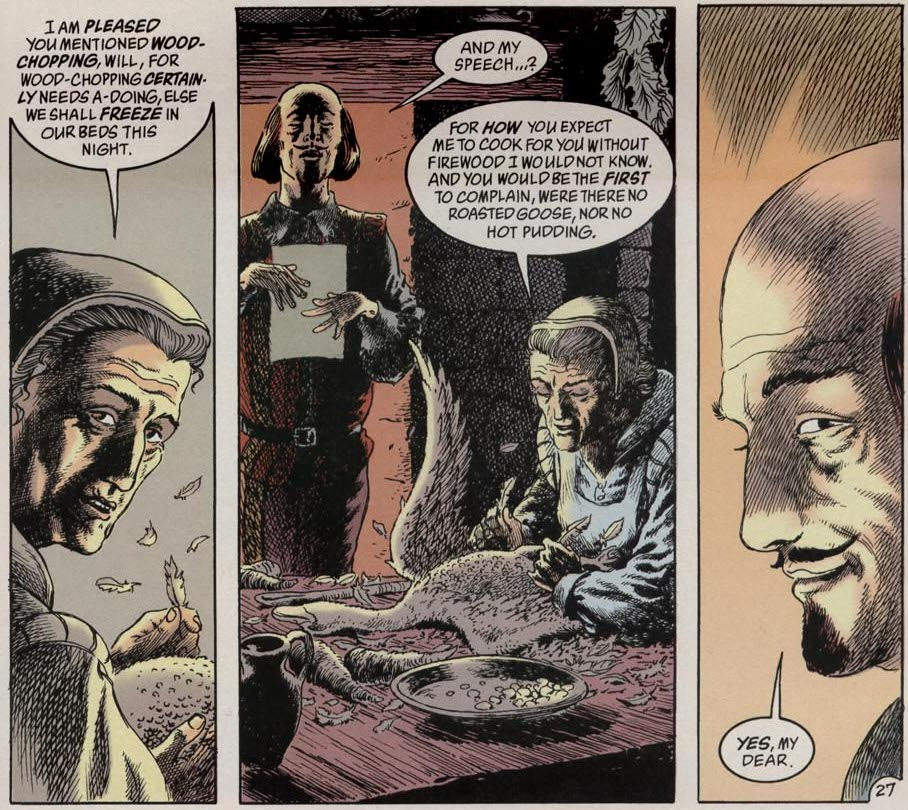
\includegraphics[scale=0.4]{../Presentation/nagging.jpg}
  \end{center}
  \caption{Nagging Wife}
  \label{nag}
\end{figure}

Gaiman also suggests that Shakespeare put in events and experiences from his own life into \emph{The Tempest}. In particular, he is shown to model Miranda after his own daughter Judith(Figure \ref{judith}), and his own feeling of protection towards Judith tranform into the overprotective father Prospero. Towards the end, Prospero is shown to renounce his magic, and Shakespeare is shown to cease writing. 

\begin{figure}[htp]
\begin{center}
  \centering
  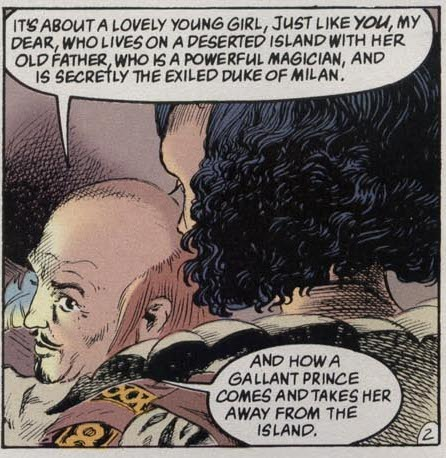
\includegraphics[scale=0.6]{../Presentation/judith.jpg}
  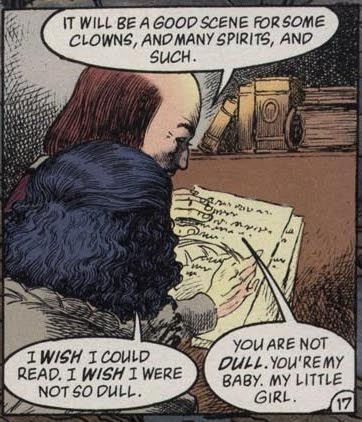
\includegraphics[scale=0.6]{../Presentation/judith2.jpg}
\end{center}
\caption{Shakespeare and Judith}
\label{judith}
\end{figure}


Another theme that Gaiman discusses is the Universality and Immortality of Shakespeare. As Gaiman points out, drama was not treated as high art in the times of Shakespeare. Though plays were extremely popular, a playwright's profession was not seen as a respectable one. This is perhaps a commentary on the status of comic books in the present. 


\begin{figure}[htp]
  \begin{center}
    \centering
    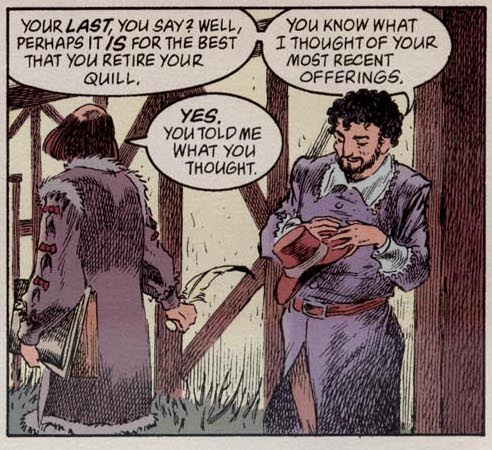
\includegraphics[scale=0.4]{../Presentation/ben.jpg}
    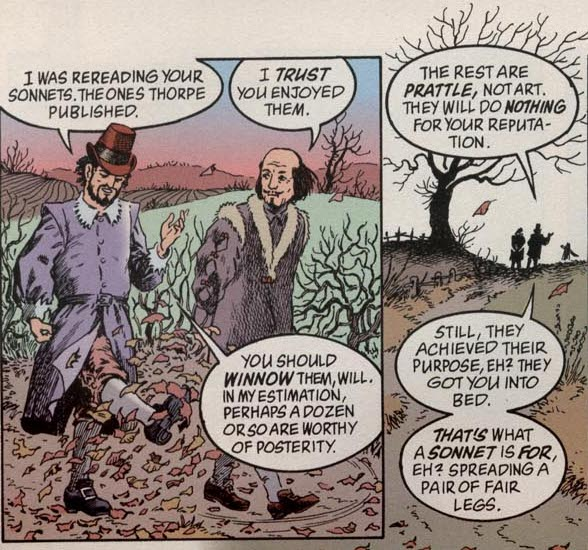
\includegraphics[scale=0.4]{../Presentation/ben2.jpg}
  \end{center}
\end{figure}

A conversation between Ben Jonson and Shakespeare is shown, where Jonson claims that one needs to experience different kinds of situations and professions in order to be able to write about them. Shakespeare's responds saying that, ``All one needs to understand people is to be a person''. Gaiman seems to say that this acute understanding of the pulse of human nature and emotions is what makes Shakespeare appealing and relevant, even today. 

\section{Discussion}
The greatness of Shakespeare is evident from the fact that he is still found interesting and relevant --- 400 years after his death. However, like any other playwright of his time, Shakespeare too was a slave of the quirks of production of a play, and he wrote the play to be performed, and not as a piece of literature to be canonized 400 years into the future. This raise a question of whether there really is a point to analysing Shakespeare to death, when in reality there may not be as much meaning or depth intended by Shakespeare. However, the very fact that we can find relevance in his work today shows us the greatness of his work. Whether he intended to portray the colonial discourse in \emph{The Tempest} is then a futile question, since if we can find it in the text, and learn lessons from it, then Shakespeare is important, and studying his works is a useful excercise. 

  \footnotesize{
    \bibliographystyle{abbrv}
    \bibliography{report}
  }

\end{document}
